\documentclass[a4paper,12pt]{report}
% Title Page
\usepackage{ctex}
\usepackage{amsmath}
\usepackage{autobreak}
\usepackage{geometry} 
\usepackage{subcaption}
\usepackage{graphicx}
\geometry{left=25mm,right=20mm,top=25mm,bottom=25mm}
\makeatletter
\newcommand{\rmnum}[1]{\romannumeral #1}
\newcommand{\Rmnum}[1]{\expandafter\@slowromancap\romannumeral #1@}
\makeatother
\usepackage{fancyhdr}
\fancypagestyle{plain}%
\fancyhf{} % 清空当前设置
		% 设置页眉 (head)
\fancyhead[LO,LE]{2020年2月天文题目汇总整理}
\fancyfoot[RO,RE]{使持节都督天文奥赛复习充电站诸军事 撰}
\renewcommand{\headrulewidth}{0.7pt} % 页眉与正文之间的水平线粗细
\renewcommand{\footrulewidth}{0.7pt}
\pagestyle{fancy} % 选用 fancy style
\usepackage{tikz}
\usepackage{xcolor}
\usepackage{eso-pic}
\usepackage{ctex}
\title{2020年2月天文题目汇总整理}
\author{使持节都督天文奥赛复习充电站诸军事}
\date{2023年1月5日}
\begin{document}
\maketitle

\chapter{数据表}
圣彼得堡地理经纬度:$\left(30^\circ25^\prime E,59^\circ55^\prime N)\right.$

1天文单位=$1.495979\times{10^{8}} km$

月球:直径3476km,平均轨道半径384403km,表面平均反照率7$\%$

地球:黄赤交角$ 23^\circ 26^\prime 21^{\prime\prime}$,平均轨道半径1AU,

轨道偏心率0.07,质量$ 5.976\times{10^{24}} $kg。

火星:平均轨道半径1.52AU,赤道半径3369km,表面平均反照率$15\%$。

太阳:半径$ 6.9599\times{10^{5}}km $,质量$ 1.989\times{10^{30}}kg $

光速:$c=299792458 m/s$

木星:半径74192km,轨道半长轴5.203AU,质量$1.90\times{10^{27}}kg$。

土星:半径60268km,轨道半长轴9.537AU,质量$5.6846\times{10^{26}}kg$。

木卫一(Io)轨道半长轴:422000km。

土星卡西尼环缝(A环和B环之间)宽度4800km。

1光年=$9.46\times{10^{12}}km$

1秒差距=3.26光年=$3.086\times{10^{13}}km$

万有引力常数:$G=6.67259\times{10^{-11}}N\times{m{^2}}\times{kg^{-1}}$

玻尔兹曼常数:$k=1.380662\times{10^{-23}}J\times{K^{-1}}$ 

普朗克常数:$h=6.626\times{10^{-34}}J\times{s^{-1}}$

斯特藩-玻尔兹曼常数:$\sigma=5.66956\times{10^{-8}}N\times{m^{-2}}\times{K^{-4}}$

\chapter{第一组习题}
\section{第一题}
\noindent 问题:

假设在同一地点观测,某颗小行星从半夜升出地平线到日落时上中天之间的时间间隔为八个月,求其轨道半长轴。假设小行星视运动均匀,答案以天文单位作为单位。

\noindent 解答:
根据题目叙述,该小行星从西方照(另外一种表述:日出时上中天)到东方照(另一种表述:半夜时没入地平线)的时间间隔为8个月,可知该小行星和地球的会合周期$T=\frac{4}{3}$年。设$P_{0}$,$P$分别为地球的轨道周期和待求小行星的轨道周期。显然有
\begin{equation}\label{eq1}
	\frac{2\pi}{P_{0}}\times{T}-2\pi=\frac{2\pi}{P}\times{T}
\end{equation}
代入解得$P$=4年。
根据开普勒第三定律,有:
\begin{equation}\label{eq2}
	\frac{a^3}{T^2}=1
\end{equation}
解得$a=2.52AU$。上式中,轨道半长轴使用天文单位作为单位,所有轨道周期均以"年"作为单位。
\section{第二题}
\noindent 问题:

某外星文明具有先进的观测手段和与我们完全一致的星等系统。他们利用视向速度法探测精度为0.1$m/s$,凌星法探测精度为千分之一星等。假设地球-太阳连线位于观测者视线方向且观测者位于无穷远处,地球有可能被使用这两种手段发现吗?请通过计算给出判断理由。

\noindent 解答:不能发现。给出论证如下。

视向速度法:

设太阳质量为$M$,地球质量为$m$,太阳和地球到二者质心之间的距离分别为$r_{0}$和$a$。
根据质心定义,有:
\begin{equation}\label{eq3}
	M\times{r_{0}}=m\times{(a-r_{0})}
\end{equation}
根据开普勒第三定律,可以得出:
\begin{equation}\label{eq4}
	\frac{a^3}{T^2}=\frac{G\times(M+m)}{4\pi^2}
\end{equation}
恒星绕二者公共质心旋转时的轨道速度:
\begin{equation}\label{eq5}
	v=\frac{2\pi{r_{0}}}{T}
\end{equation}
联立得到$v=0.09m/{s}^2<0.1m/{s}^2$
可知,不可以用视向速度法被发现。

凌星法:

设太阳和地球的半径分别为$R$和$r$。凌星之前的光流量为$f$,凌星时的光流量为$F$。应有
\begin{equation}\label{eq6}
	f\propto{R^2},F\propto{(R^2+r^2)}
\end{equation}
同时可以看出,
\begin{equation}\label{eq7}
	\frac{f}{F}=\frac{R^2}{R^2+r^2}
\end{equation}
根据视星等定义,凌星之前和凌星之后的视星等差应写成:
\begin{equation}\label{eq8}
	\Delta m=-2.5\lg\frac{F}{f}
\end{equation}
代入数据解得$\Delta m=9.10\times{10^{-5}}$等,显然也不能发现。

\section{第三题}

\noindent 问题:

某望远镜可记录下主带小行星中直径大约$5km$的,那么该望远镜能记录下柯伊伯带天体中半径至少为多少的?

\noindent 解答:

柯伊伯带距离太阳30$\sim$55AU,本题计算取其中位数$a_{2}=45 AU$。
小行星带距离太阳1.9$\sim$4.2AU,本题计算取其中位数$a_{1}=2.7 AU$。
太阳辐射到达两个距离的光流量之比:
\begin{equation}\label{eq9}
	\frac{F_{1}}{F_{2}}=\frac{S_{1}}{S_{2}}=({\frac{a_{1}}{a_2}})^2=\frac{2500}{9}
\end{equation}
在地球上,如果只考虑二者冲日时最亮的主带小行星,从以上两处返回地球的光流量之比:
\begin{equation}\label{eq10}
	\frac{F^{\prime}_{1}}{F^{\prime}_{2}}=({\frac{a_{2}-1}{a_{1}-1}})^2	
\end{equation}
同样反照率条件下,同样大小的主带小行星和柯伊伯带天体反射到地球上的光流量之比:
\begin{equation}\label{eq11}
	\frac{F^{\prime\prime}_{1}}{F^{\prime\prime}_{2}}=\frac{S_{1}}{S_{2}}\times\frac{R_{1}}{R_{2}}	
\end{equation}
二者直径之比和反射太阳光的表面积之比,不难发现:
\begin{equation}
	r_{1}=r_{2}\times \sqrt{\frac{S_{1}}{S_{2}}}
\end{equation}
代入数据不难计算,可以看到柯伊伯带天体中半径至少为$1078.43km$的。
\section{第四题}
问题:

\noindent 在某星系中发现一颗极亮时绝对星等$-19.5$等的$\Rmnum{1}a$型超新星,测得该星系红移为$0.03$,该超新星视星等为$15.5$等。不考虑星际消光和宇宙学红移,试估算哈勃常数。

\noindent 答案:

\noindent 根据距离模数公式可得:
\begin{equation}\label{eq}
	m=M=5lgr-5
\end{equation}
得出$r=100 Mpc$

\noindent 根据相对论条件下的红移严格表达式:
\begin{equation}
	v=\frac{(z+1)^2-1}{(z+1)^2+1}=6815.95km/s
\end{equation}

\noindent 根据哈勃定律,有:
\begin{equation}
	H=\frac{v}{r}=68.16km/s/Mpc
\end{equation}

\section{第五题}

\noindent 问题:

\noindent 请估算全天六千多颗肉眼可见的恒星中有多少颗在赤道以北$1^\circ$的地区。

\noindent 答案:

\noindent 根据常识,全天面积41253平方度。

\noindent 球冠高度:
\begin{equation}
	h=R-R\sin{1^\circ }
\end{equation}
\noindent 球冠面积:
\begin{equation}
	S=\pi \times(h^2+R^2)
\end{equation}
\noindent 此范围内所有肉眼可见的恒星数目(本题假设全天所有肉眼可见的恒星在天球上的分布是均匀的。)
\begin{equation}
	6000\times \frac{20445}{41253}=2695
\end{equation}

\section{第六题}
\noindent 问题:

有一台焦距$F=1000mm$,口径$D=100mm$的望远镜。

\noindent $\left(1\right)$求观测视直径$31^\prime$的月球时,像在焦平面上所成的像大小。

\noindent $\left(2\right)$该望远镜使用全画幅相机进行照相巡天,在赤道上放置的这套设备理论上需要拍摄多少张照片才能达到预定目的?

\noindent $\left(3\right)$在可见光波段工作的这套设备能否用目视的方式分辨出木星的四颗伽利略卫星和土星的卡西尼环缝?请通过计算论证。忽略大气的影响。

\noindent 答案:

\noindent $\left(1\right)$
\begin{equation}
	x=f\tan {\theta}=1000mm\times \tan(31^{\prime\prime})=9.02mm
\end{equation}
$\left(2\right)$
底片比例尺

\begin{equation}
	\alpha=\frac{206265}{F}=206.265(sec/mm)
\end{equation}
\noindent 根据常识,全画幅相机传感器的尺寸为36mm$\times$24mm。

\noindent 则长边对应视场大小:$36mm \times206.265(sec/mm)= 7425.54^{\prime\prime}$

\noindent 短边对应的视场大小:$24mm\times 206.265(sec/mm)=4950.36^{\prime\prime}$

\noindent 视场的范围大小:$S=2.8634$平方度。

\noindent 全天总面积:$S_{0}=41253$平方度。

\noindent 需要拍摄的数量 
\begin{equation}
	n_{0}=\frac{S_{0}}{S}=14545
\end{equation}

\noindent 可知需要14545张照片。

\noindent $\left(3\right)$
\noindent 根据常识,人眼目视有效波长$\lambda = 555 nm$。此时,题中望远镜的分辨角$\delta = 1.4^{\prime\prime}=6.787\times 10^{-6}rad$。

\noindent 在木星的伽利略卫星中,木卫一距离木星最近。
认为其轨道半径421700km。

\noindent 在地球上的木星冲日前后,记木星和木卫一张角为$\theta$。

\noindent 根据三角函数定义可以写出,$tan\theta = \frac{42200km}{(5.203-1)AU}=7.012\times 10^{-4}$, 因此此时可以分辨。

\noindent 在地球上的土星冲日前后且土星的光环垂直于观测者的视线时,记土星卡西尼环缝间的视角为$\beta$。

\noindent 根据三角函数的定义同样可以写出,$tan\beta = \frac{4800km}{(9.537-1)AU}=3.759\times 10^{-6}$,
故不可以分辨。
\section{第七题}
\noindent 问题:

某直径0.1光年的星云碎块每百万年旋转一周,开始坍缩。若其质量不变,求它收缩至太阳系尺度$\left(50AU\right)$之时的自转周期。

\noindent 答案:

\noindent 根据角动量守恒定律,有:

\begin{equation}
	mr_{1}^2\omega_{1}=mr_{2}^2\omega_{2}
\end{equation}

\noindent 整理,有
\begin{equation}
	\frac{r_{1}^2}{T_{1}}=\frac{r_{2}^2}{T_{2}}
\end{equation}

代入得$T_{2}=15813.73$年。




\section{第八题}
问题:

某次火星冲日期间,为测定地-火距离,甲在圣赫勒拿岛,乙在摩尔曼斯克同步展开观测。当二人连线垂直于地球-火星连线时,发现二者记录的火星相对于地区的投影位置有$26^{\prime \prime}$的差别。不考虑地球、火星的轨道偏心率,求此时火星到地球的距离是多少天文单位?地球视作半径6371$km$的正球体。

圣赫勒拿岛:$\left(5^\circ42^\prime W,15^\circ56^\prime S)\right.$

摩尔曼斯克:$\left(33^\circ03^\prime E,68^\circ58^\prime N)\right.$

\noindent 答案:
本题答案暂缺。
\noindent 解球面三角形,得到地心位置处看,甲乙两人所在地的张角满足以下关系式。


地理坐标:A$\left(33^\circ3^\prime E,0^\circ)\right.$,B$\left(5^\circ42^\prime W,15^\circ56^\prime S)\right.$,

C$\left(33^\circ3^\prime E,15^\circ56^\prime S)\right.$D$\left(33^\circ3^\prime E,68^\circ58^\prime N)\right.$

解球面三角形ABC。三边分别为a,b,c。
\begin{equation}
	\cos15^\circ56^\prime =\cos c\cos(5^\circ42^\prime+33^\circ3^\prime)+\sin(5^\circ42^\prime+33^\circ3^\prime)\sin c\cos B
\end{equation}
\begin{equation}
	\cos 90^\circ \sin 15^\circ56^\prime=\cos c\sin )(5^\circ42^\prime+33^\circ3^\prime)-\sin c\cos(38^\circ45^\prime)\cos B
\end{equation}
联立解得
\begin{equation}
	\cos c=\frac{\cos  15^\circ56^\prime}{(1+\tan 38^\circ45^\prime)\cos 38^\circ45^\prime}
\end{equation}


解球面三角形ABD。记$BD=f$,$AD=e$。
$\sin DAB =\frac{\sin f}{\sin c}$
根据球面三角形边的余弦公式,代入之后应有:
\begin{equation}
\begin{split}
	\cos f=\sin{\arccos[\frac{\cos15^\circ56^\prime}{(1+\tan 38^\circ45^\prime)\cos 38^\circ45^\prime}]}\sin68^\circ58^\prime\cos[\arcsin(\frac{\sin15^\circ56^\prime}{\sin38^\circ45^\prime})+90^\circ]\\
	\noindent +\frac{\cos  15^\circ56^\prime}{(1+\tan 38^\circ45^\prime)\cos 38^\circ45^\prime}\cos68^\circ58^\prime 
\end{split}
\end{equation}
\noindent $\cos f=-0.05312075504$
	
\noindent $f=93.0450283^\circ$
	
\noindent 记两人所处位置之间的直线距离为$d$。d满足:
\begin{equation}
	\frac{d}{2}=(6371km\times \sin(\frac{f}{2}))
\end{equation}
有$d=9246.166057$km。
$26^\prime$是火星相对于基线的视差。可知,在冲日时火星距离地球的距离:
\begin{equation}
	r=\frac{d}{\frac{25^{\prime\prime}}{206265^{\prime\prime}}}=0.49AU
\end{equation}

\section{第九题}
\noindent 问题:

请估算一只猫的绝对星等。

\noindent 答案:

\noindent 根据斯特藩-玻尔兹曼定律,将猫和太阳均视作绝对黑体,有
\begin{equation}
	\frac{L_{cat}}{L_{sun}}=\frac{S_{cat}}{S_{sun}}(\frac{t}{T})^4
\end{equation}
\noindent 一只猫的表面积为0.15平方米,可以得出$\frac{L_{cat}}{L_{sun}}=2.196\times 10^{-25}$

\noindent 根据光度和星等的关系,得到:
\begin{equation}
	M_{cat}-M_{sun}=-2.5\lg\frac{L_{cat}}{L_{sun}}=61.646
\end{equation}

\noindent 得到猫的绝对星等:$M_{cat}=66.48$

\section{第十题}

\noindent 问题:不考虑地球大气层,在地球上何时何地可以观测到最长时间约为多少的日出?

\noindent 答案:
\noindent 南北两极春分和秋分可以看见最长的日出。以下计算忽略大气折射与大气消光。
在北极点,地平圈和天赤道重合,黄道和地平圈的夹角为$\epsilon$。春分点可以认为在地平线上。

太阳在黄道上运动的角速度:

\begin{equation}
	v=\frac{360^{\circ}}{365.2422day}=0.986^{\circ}/day
\end{equation}

太阳的视直径为$15^\prime $,日出过程即为太阳视中心的地平高度从$-15^\prime$变为$+15\prime$的过程。

所用时间
\begin{equation}
	t=\frac{2\times15^\prime\frac{1}{sin(\epsilon)}}{0.986^\circ/day}=1.28days
\end{equation}
此处可以认为春分前后太阳运动轨迹大致为直线。

同理,北极点的秋分、南极点的春分秋分时观察到的日出时间都是最长的。计算得到的时间相同。

\chapter{第二组}
\section{第一题}
\noindent 问题:一千颗视星等为8等的恒星聚集在一起,试估算其星等。

\noindent 解答:

对于单颗恒星
\begin{equation}
	m_{1}=8^m=-2.5\lg E_{1}
\end{equation}
对于该恒星系统中所有的恒星
\begin{equation}
	m=-2.5 \lg E=-2.5 \lg (E\times1000)=-2.5\lg E_{1}-2.5\lg 1000 
\end{equation}
则:
\begin{equation}
	m=m_{1}-2.5\lg 1000=m_{1}-7.5^m=0.5^m
\end{equation}
则总星等为0.5等。

\section{第二题}
\noindent 问题:某个由相似的恒星组成的星团,在赫罗图上的位置约为-7$\sim$-8等。星团的光谱型为A0。请估算该星团中恒星的数目。

\noindent 解答:
根据常识,光谱型为A0的恒星,其绝对星等为0等。

\begin{equation}
	M_{1}\sim -2.5 \lg L=0
\end{equation}
\begin{equation}
	M_{2}\sim -2.5\lg(N\times L)=-2.5\lg N
\end{equation}
根据已知,绝对星等为-7$\sim$-8等,该星团内有600$\sim$1600颗恒星。
\section{第三题}
\noindent 问题:水星的自转轴垂直于公转轨道平面,其自转周期是其公转周期的三分之二。求在水星上观测,日出到日落经过多少个水星日?

\noindent 解答:

根据已知,水星上的日夜长度相等。设$T_{s}$为水星的自转周期,$T_{0}$为水星的公转周期。一个水星日的长度为$t$。由于水星的公转和自转周期相同,若想连续看到太阳升起,水星除了完成一次自转,还必须转过一个角度将公转造成的减少补回来。假设这个角度:
\begin{equation}
	\alpha=\frac{2\pi t}{T_{0}}
\end{equation}
转动这$\alpha$角度需要额外花费的时间:
\begin{equation}
	\Delta T=T_{s}\times \frac{\alpha}{2\pi}
\end{equation}
在一个水星日内,水星转动的总时间应当写成
\begin{equation}
	t=T_{s}+T{s}\frac{t}{T_{0}}
\end{equation}
联立以上各式可得$t=2T_{0}$。
据此得知,水星从日出到日落的时间是一个水星年

\section{第四题}
\noindent 问题:对某近日点2天文单位,远日点5天文单位的小行星进行两次观测,观测当天太阳高度角为零时该小行星的地平高度角同样为零。两次观测时,该小行星一次位于近日点,另一次位于远日点。忽略地球的轨道偏心率,求这两次观测时小行星的星等差。

\noindent 解答:
根据题目叙述,该小行星应该在合或冲时,才能达到太阳高度角为$0^\circ$时,该小行星的地平高度同样为$0^\circ$。当该小行星合日时,和太阳同时升起、同时落下,不能观测。因此题目中两次观测全部位于小行星冲日时进行。

若一颗到太阳和地球距离分别为$a$和$b$的小行星,根据平方反比定律,经太阳到小行星再到地球的光流量应该满足:
\begin{equation}
	F\sim \frac{1}{a^2 b^2}
\end{equation}
第一次冲日时,$a_{1}=2AU,b_{1}=2AU-1AU=1AU$
第二次冲日时,$a_{2}=5AU,b_{2}=2AU-1AU=4AU$
根据星等的定义,两次观测时的星等差:
\begin{equation}
	\Delta m =m_{2}-m_{1}=-2.5\lg \frac{F_{2}}{F_{1}}=-2.5\lg \frac{(a_{1}b_{1})^2}{(a_{2}b_{2})^2}
\end{equation}
计算得出两次观测的星等差为5等。
\section{第五题}
\noindent 问题:在冬至日,源PSR J1748-2446何时上中天?(精确到小时。)

\noindent 解答:题中符号表示一个在2000.0历元下,赤经$\alpha =17^h 48^m$,赤纬$\delta = -24^\circ 06^\prime$的射电源。
太阳在冬至日时的赤经约为18h,则此射电源上中天的时间和太阳上中天的时间相近,为地方时12h。
\section{第六题}
\noindent 问题:在当地时间某日午夜零时,某天文爱好者在拍摄星轨时发现天权和天枢在北极星正上方几乎连成正南正北的一条线。已知天枢的赤道坐标$\alpha=11^h 4^m, \delta = 61^\circ 45^\prime $,请推算可能的拍摄日期。

\noindent 解答:
根据已知,该观测者拍摄时地方恒星时和天枢的赤经相等。即$S_{1}=11^h4^m$。此时地方平时$t=0h$。根据常识,每年秋分日地方时零时应有$S_{2}=t$。由于恒星日和平太阳日每天相差3分56秒,这一天的日期和秋分相差:
$\Delta t=\frac{11^h4^m}{3^m56^s}=169$天。可以看出拍摄日期大约为3月11日左右。
\section{第七题}
\noindent 问题:一颗白矮星的半径为6000千米,表面温度为$10^5 K$,质量与太阳质量相等。当它穿过一团星际彗星云时,会因为彗星落在表面而亮度增大。如果云内每颗彗星的半径为1千米,密度和水的密度相当。若白矮星亮度增加到原来的二倍,每天约有多少颗彗星落到它的表面?若白矮星的质量达到钱德拉塞卡极限,成为$\Rmnum{1}a$型超新星并爆发,按照此速度计算需要多长时间?假设该星际彗星云足够大,且彗星云中各处彗星始终分布均匀,白矮星可以在其中停留足够长的时间。

\noindent 解答:

\noindent $(\Rmnum{1})$
该白矮星的光度:
\begin{equation}
	L=4\pi R^2\sigma (T)^{4} = 2.5648\times 10^{23} W
\end{equation}
在一天,86400秒之内,白矮星释放出的能量
\begin{equation}
	E=L\times t=2.2160\times 10^{28} J
\end{equation}
单个彗星的彗核质量:
\begin{equation}
	m=\frac{4}{3}\pi r^3\rho=4.18879\times 10^{12} kg
\end{equation}
单个彗核在落向白矮星表面的过程中,仅考虑引力势能的释放过程,释放出的能量:
\begin{equation}
	E_{0}=\frac{GMm}{R}=9.26545\times 10^{25} J
\end{equation}
假设每天能有$n$颗彗星落到表面。如果彗星落到白矮星表面提供的能量和白矮星的光度相当。
\begin{equation}
	n=\frac{E_{0}}{E}=240
\end{equation}
即每天应约有240颗彗星落到白矮星表面。

\noindent $(\Rmnum{2})$
每天当中白矮星的质量增量:
\begin{equation}
	\Delta m = n\times m=1.0053\times 10^{15}kg
\end{equation}
根据常识,钱德拉塞卡极限(1.44倍的太阳质量)是白矮星的质量上限。设经过的时间(使用儒略年作为单位)为$\tau$,则:
\begin{equation}
	(\tau \times 365.25)\times \Delta m=M_{c}-M_{s}
\end{equation}
得出$\tau =2.38\times 10^{12}$儒略年。显然,白矮星在成为$\Rmnum{1}a$型超新星并发生超新星爆发之前已经冷却。所求时间不存在。

\section{第八题}
\noindent 问题:月全食时的月球视星等为1.865等,求全食的持续时间。忽略由大气原因导致的地球本影增大。

\noindent 解答:
假设食甚时,太阳、地球、月球严格共线。

\noindent 用日地距离$L$和地月距离$l$表示本影半径$\rho$:
本影锥的母线与太阳-地球中心连线呈一角度:
\begin{equation}
	\gamma = \frac{S-R}{L}
\end{equation}
上式中取太阳半径为$S$,地球半径为$R$。根据近似公式,取$\sin \gamma=\gamma $,$\cos \gamma =1$。
本影的半径为:
\begin{equation}
	\rho=R-\gamma L=\frac{R(L+l)-Sl}{l}
\end{equation}
通过作图不难发现,食甚时的视星等为:
\begin{equation}
	F=1+\frac{d}{2r}=1+\frac{\rho-r}{2r}=\frac{\rho+r}{2r}
\end{equation}
其中,$r$为从地球上看,月球的角半径;$d$为月球视圆面和地球本影边缘的距离(所在直线是两圆公共直径所在的直线。)。
显然,日地距离$L$越大且地月距离越小,食星等越大。若月食发生时地球位于公转轨道上的远日点($L=1.017AU$),先假设$l$为其平均值384000km,和题中发生情况不符。
在忽略大气层影响的前提下,可观测到的最大食星等为1.868等,所以,题中叙述的情况发生在月球经过近地点,本影半径为4757km。根据活力公式,得出月球在距离地心$l$处的运行速度
\begin{equation}
	v=\sqrt{GMm(\frac{2}{r}-\frac{1}{a})}
\end{equation}
其中,$a$为月球轨道半长轴,$v_{0}$为地球在远地点的速度,同样可以通过对应的活力公式得到$v_{0}=29.3km/s$。
本影相对于地球的运动速度:
\begin{equation}
	u=\frac{v_{0}l}{L}=0.069km/s
\end{equation}
$u$,$v_{0}$的方向相同,
月全食过程中月球运行的距离:
\begin{equation}
	D=2(\rho-r)
\end{equation}
月全食的持续时间:
\begin{equation}
	t=\frac{D}{v-u}=\frac{2(\rho -r)}{v-u}=1h38.1m
\end{equation}
本题答案应为食星等略小于最大值的月食持续时间。

\section{第九题}
\noindent 问题:柯克伍德空隙。

$\left(1\right)$
有一个柯克伍德空隙,其中小行星和木星的会合周期等于木星的公转周期,求这个柯克伍德空隙距离太阳的距离。

$\left(2\right)$
由于木星的引力作用,此空隙上的一颗小行星被拽到了比圆轨道半径长$\Delta r = 0.01AU $的轨道上。若某年春分日观测到小行星和太阳同升同落,求小行星能够在半夜升出地平的日期。

\noindent 解答:

\noindent $\left(1\right)$
根据会合周期公式,有:
\begin{equation}
	\frac{1}{T_{0}}=\frac{1}{T_{a}}-\frac{1}{T_{J}}
\end{equation}
解得会合周期:$T_{0}=5.93$年。

在轨道半长轴取天文单位作为单位,公转周期以"年"作为单位时,开普勒第三定律可以写成:
\begin{equation}
	\frac{a^{3}}{T_{0}^2}=1
\end{equation}

解得$a=3.2762AU$,即为所求。

\noindent $\left(2\right)$
设小行星原来的轨道周期和新的轨道周期分别为$T$,$T+\Delta T$;原轨道半径和新的轨道半径分别为$r$,$r+\Delta r$。
根据开普勒第三定律可以写出:
\begin{equation}
	\frac{r^3}{T^2}=\frac{(r+\Delta r)^{3}}{(T+\Delta T)^{2}}
\end{equation}
考虑到 $\Delta T$和$\Delta r$都甚小,使用近似公式,可以改写成:
\begin{equation}
	\frac{3\Delta r}{r}=\frac{2\Delta T}{T}
\end{equation}
代入解得$\Delta T=0.02715$年,
新的轨道周期:$T^\prime =T+\Delta T=5.95715$年。
当小行星在半夜升出地平,所在位置为西方照。设地球和小行星的会合周期为$t$,地球轨道周期为$T_{0}$,可以方便地得出:
\begin{equation}
	\frac{1}{t_{0}}=\frac{1}{T^\prime}+\frac{1}{t}
\end{equation}
据此解出$t=1.2017$年。假设小行星在黄道上视运动是均匀的,则由合日到西方照的时间为其会合周期的四分之一,即0.3年。折合109.5天。从春分日向后推算,待求日期为7月9日。需要指出,此结果因春分日期的不确定可有前后各一天的误差。
\section{第十题}
\noindent 问题:如果通过改变月球的轨道使得地球上的人处于"永恒的日食"当中,月球质量保持不变,求月球密度应为现在的多少倍。

\noindent 解答:

若要求处于永久的日食状态,月球必须在日地之间且一定位于日地拉格朗日$L1$点上。此处,地球绕太阳公转的角速度和月球绕地球公转的角速度应当相等,即
\begin{equation}
	\omega_{earth}=\omega_{moon}=\omega
\end{equation}
假设月球质量、太阳质量和地球质量分别为$m$,$M$,$M_{0}$。
假设地月距离$D_{1}$,日地距离$D$。
对月球,地球和太阳施加的万有引力的合力提供月球绕转地球所需的向心力。
即:
\begin{equation}
	\frac{GMm}{(D-D_{1})^2}-\frac{GM_{0}M}{D_1^{2}}=\omega^2m(D-D_{1})
\end{equation}
考虑到$M_{0} \ll M$,$D \gg D_{1}$,

可以写为:
\begin{equation}
	\frac{GM}{(D-D_{1})^2}=\frac{GM}{D^2}+\frac{2GMD_{1}}{D^3}
\end{equation}
\begin{equation}
	\frac{GM}{D^2}+\frac{2GMD_{1}}{D^3}-\frac{GM_{0}}{D_1^{2}}=\omega ^2(D-D_{1})
\end{equation}
日地系统之间的引力平衡:
\begin{equation}
	\frac{GM}{D^2}=\omega^2 D
\end{equation}
各表达式联立可得:
\begin{equation}
	D_{1}=(\frac{M_{0}}{3M})^{\frac{1}{3}}D=0.01AU
\end{equation}
此时,月球半径应为:
\begin{equation}
	R=R_{earth}+D(R_{sun}-R_{earth})=1.3296\times 10^{4}km
\end{equation}
根据球体体积公式及密度的定义,有:
\begin{equation}
	\rho =(\frac{r_{0}}{r})^3\rho_{0}=2.234\times 10^{-3}
\end{equation}
所以,那时的月球密度应该为现在的$2.234\times 10^{-3}$倍。
\section{第十一题}
\noindent 问题:在圣彼得堡(纬度:北纬60$^\circ$)有一固定观测点。当地地方平时为6月22日24时,对某颗正好上中天的恒星测量地平高度。该恒星的表面有效温度为6500开尔文,测量时此恒星的地平高度为$31^\circ$。在同一年的8月22日的同一时刻再次测量,当此恒星又一次上中天时,赤纬减少了$0.05^{\prime\prime}$。本题忽略大气层的影响及星际消光。回答以下问题:

$\left(1\right)$求此恒星相对于天球上遥远恒星背景移动的总角度。

$\left(2\right)$若此恒星的视星等为1.5等,半径和太阳半径相等。求它辐射最猛烈的波长。
\noindent 解答:
$\left(1\right)$
由题可知该恒星的赤经为18h。6月22日,在圣彼得堡,上中天时的地平高度满足:
\begin{equation}
	90^\circ-\lvert \delta_{0} -60^\circ \rvert=31^\circ 
\end{equation}
解得该恒星的赤纬:$\delta_{0} =1^\circ$

\noindent 利用球面三角公式将该恒星的赤道坐标转化为黄道坐标:
\begin{equation}
	\sin \beta =\cos \varepsilon \sin \delta -\sin \varepsilon \cos \delta \sin \alpha
\end{equation}
\begin{equation}
	\cos \lambda \cos \beta=\cos \alpha \cos \delta
\end{equation}
其中,$\delta =\delta_{0}+\Delta \delta=1^\circ 0^{\prime} 0.05^{\prime\prime}$。

\noindent 可以得到该恒星在8月22日观测时,黄道坐标$\lambda =0$,$\beta =65^\circ 33^\prime 38.95^{\prime\prime}$。
分别从北黄极位置俯视、从秋分点方向侧视,得到被观测恒星(S点),太阳(O点)和地球(E点)的位置关系如图所示。
\begin{figure}[!h]
	\centering
	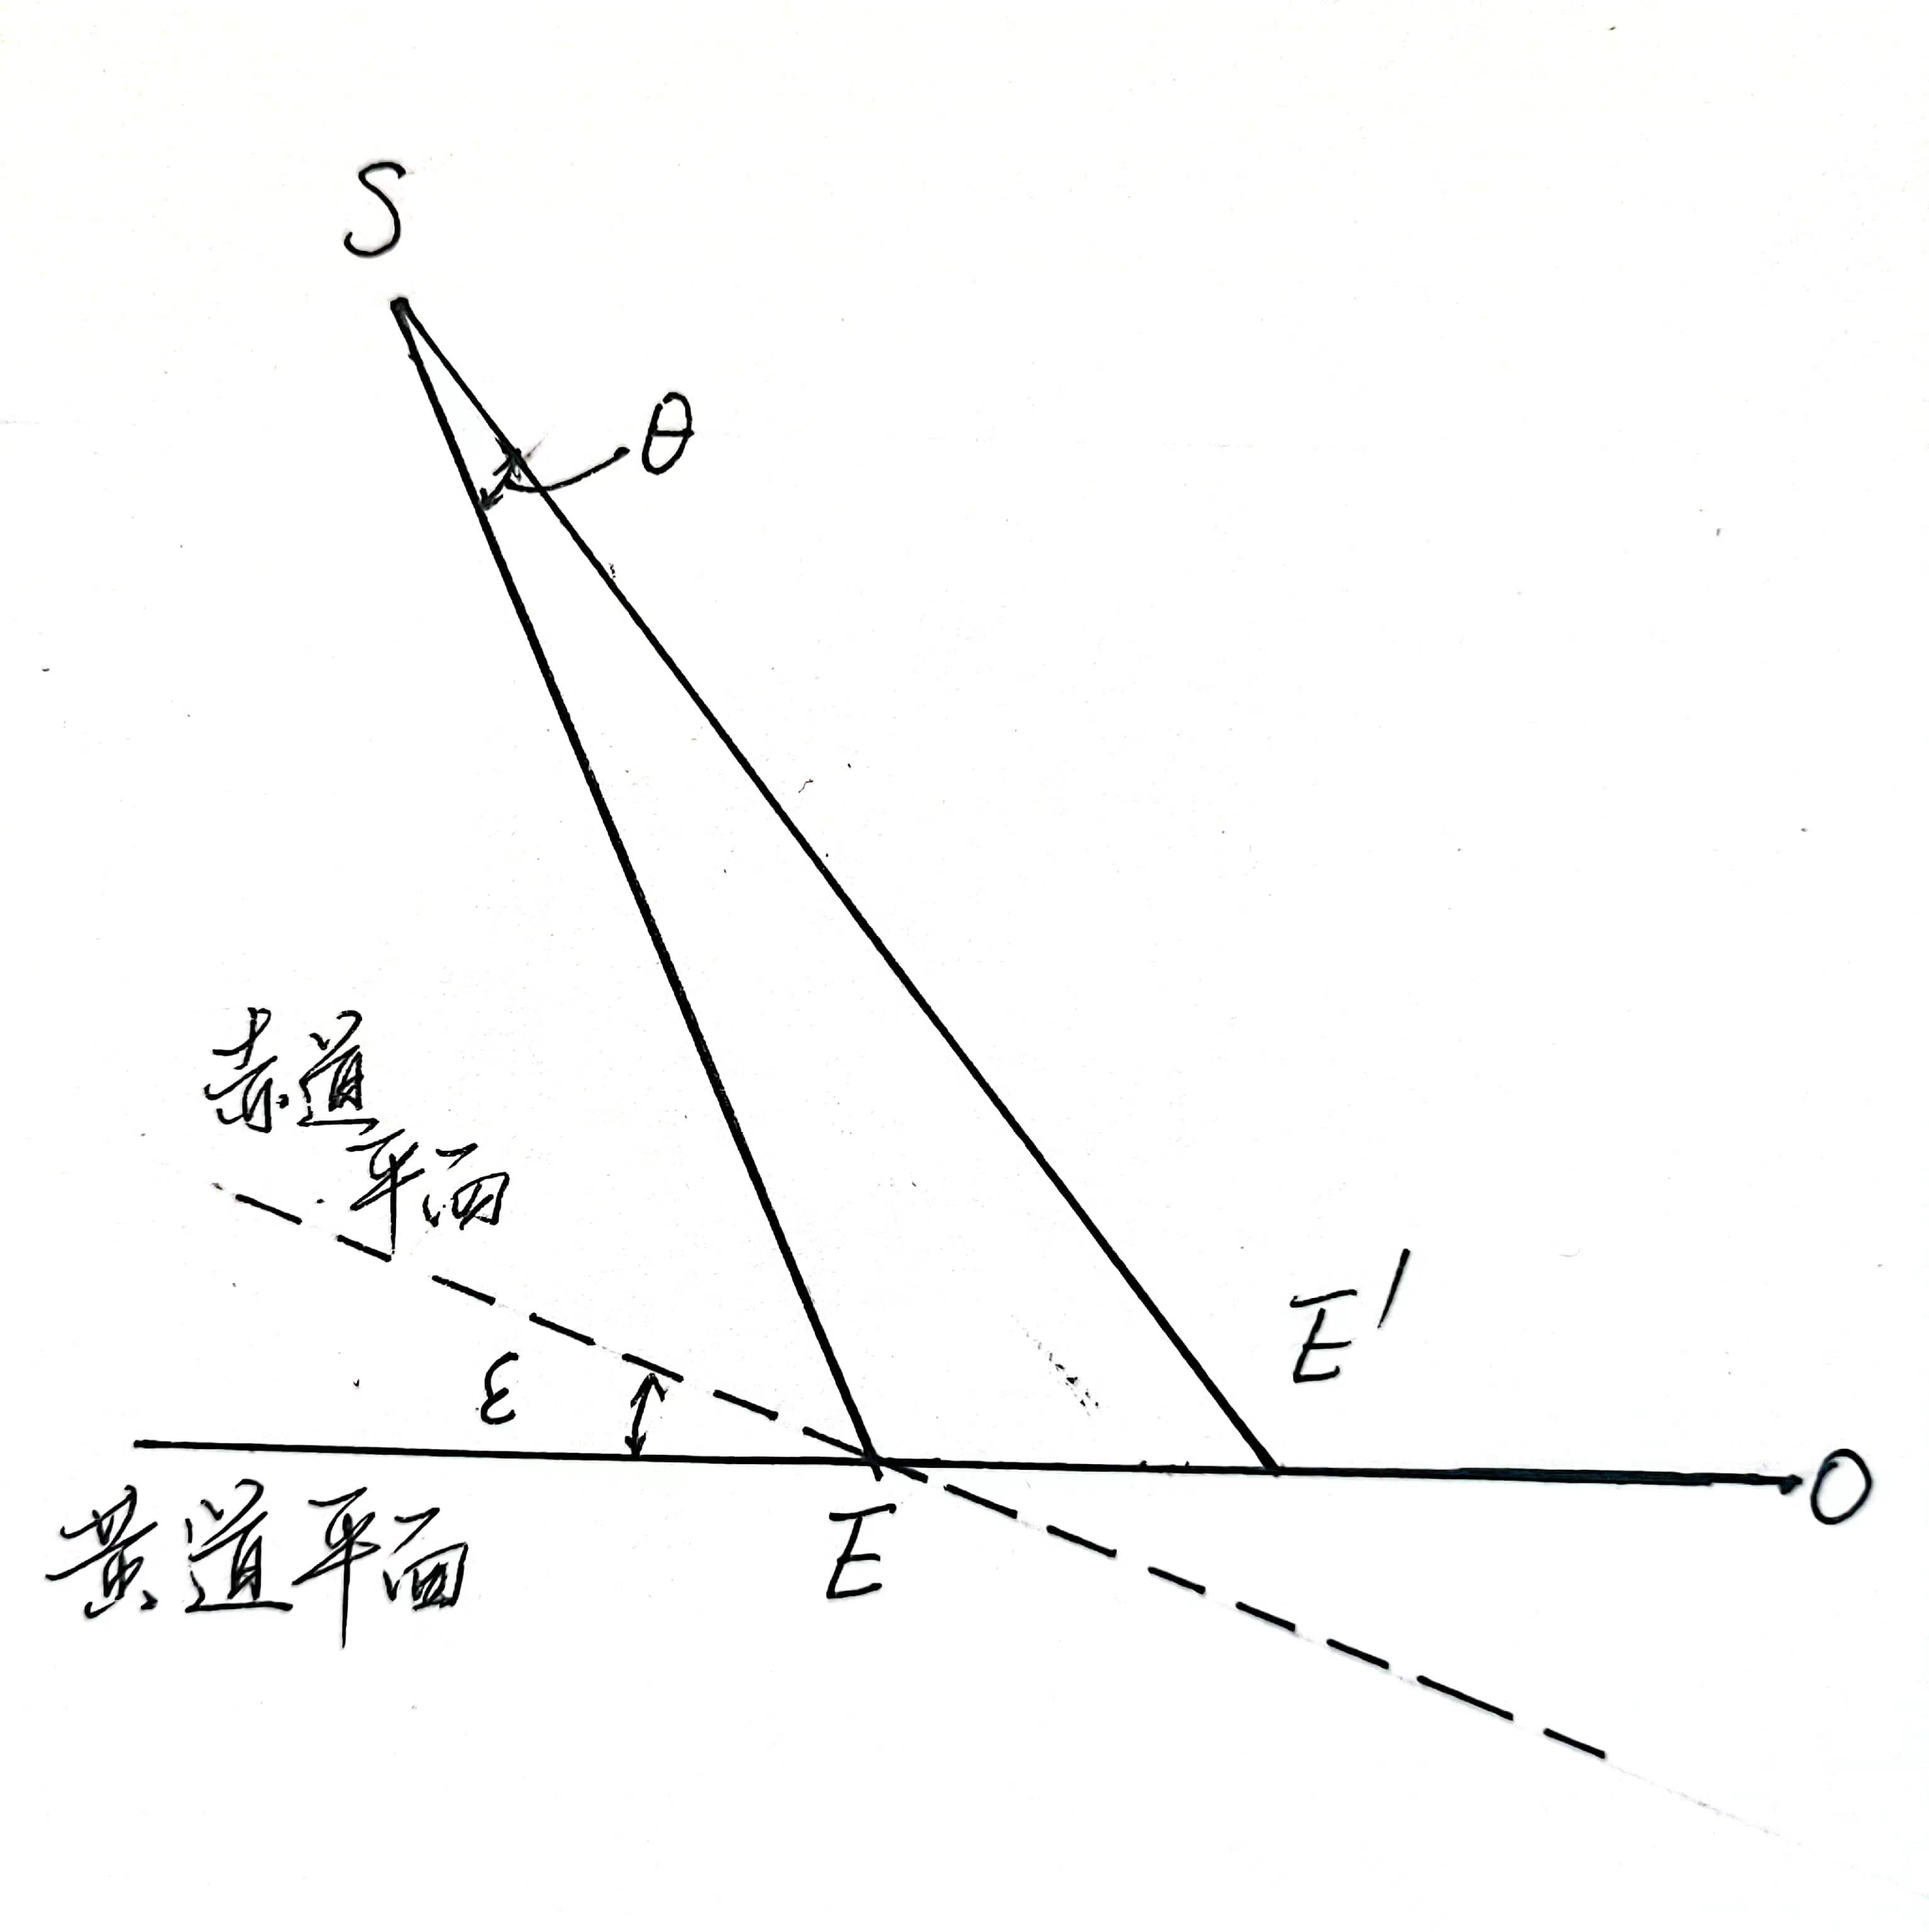
\includegraphics[width=7cm]{3_11B.jpg}
	\caption{图一}
	%\label{fig:circuit-diagram}
\end{figure}

\begin{figure}[!h]
	\centering
	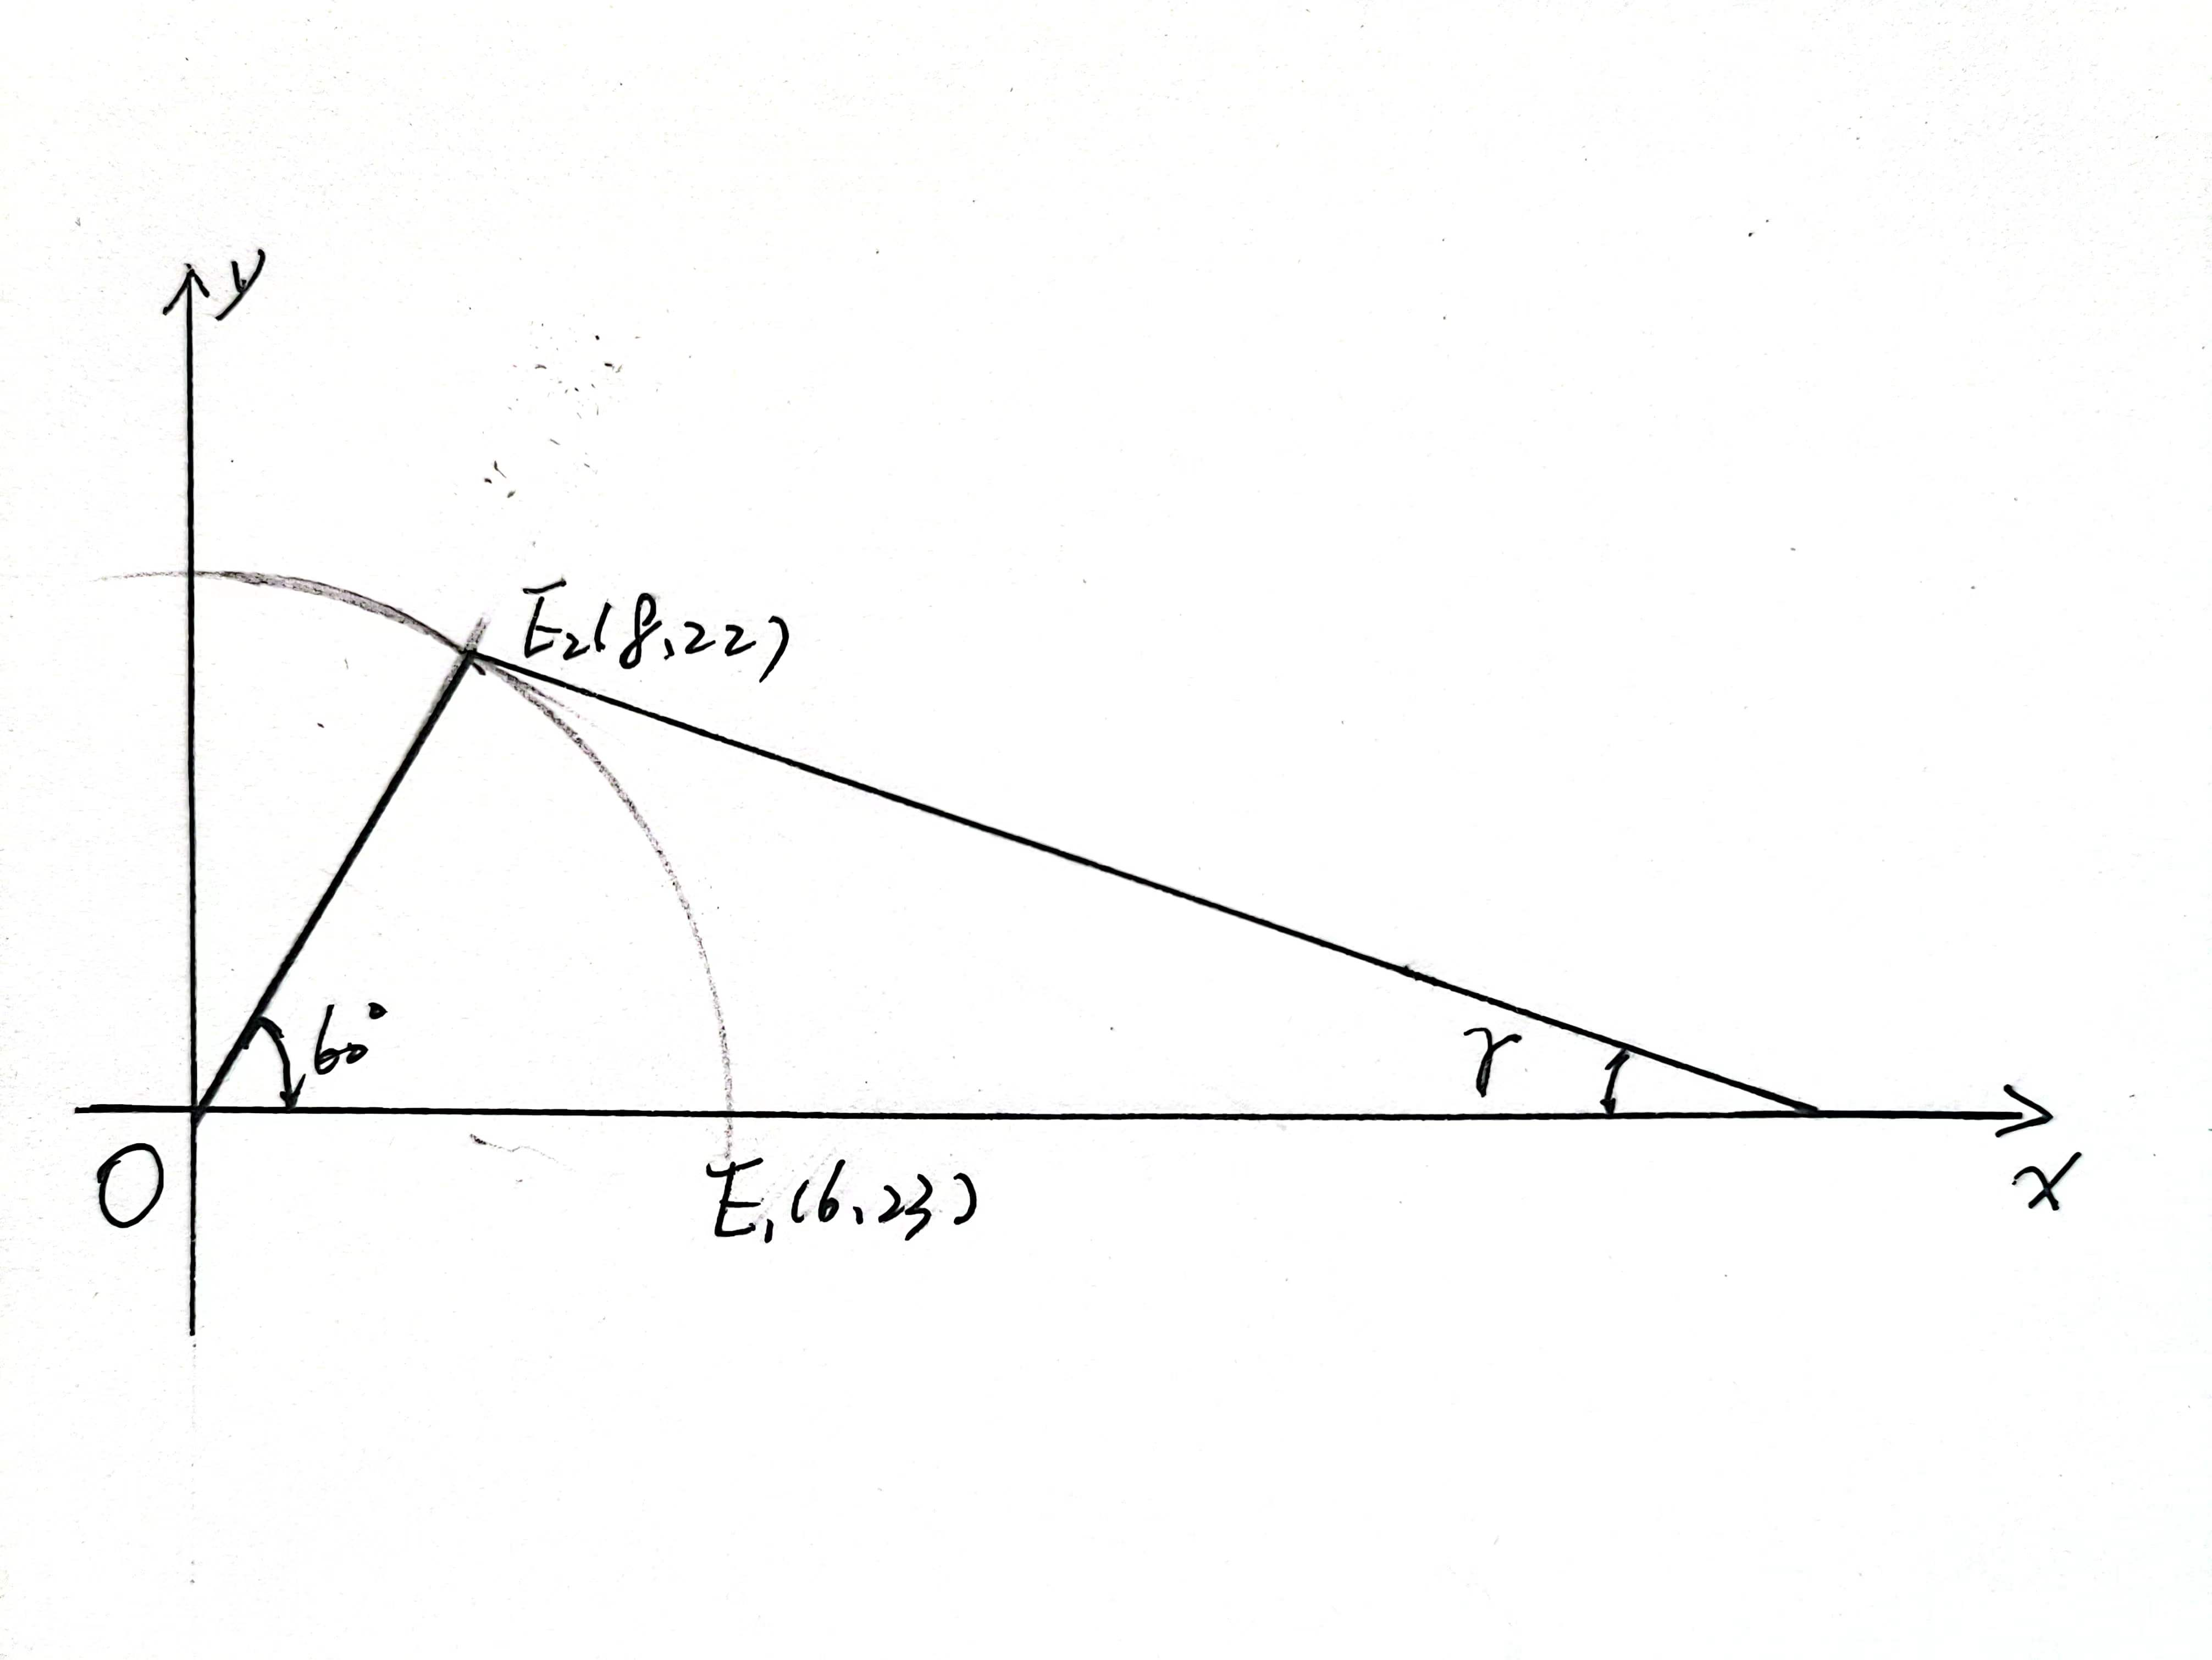
\includegraphics[width=9cm]{3_11A.jpg}
	\caption{图二}
	%\label{fig:circuit-diagram}
\end{figure}

\noindent 在图二的三角形$\triangle SEE$中,设待求距离$ES=D$,根据正弦定理应该有:
\begin{equation}
	\frac{A}{\Delta \delta}=\frac{D}{\angle SEE^\prime}
\end{equation}
解得$D=852332.3325AU$
在图一中,应有:
\begin{equation}
	\sin \gamma =\frac{\Delta y}{D}=\frac{\frac{1}{2}AU}{D}
\end{equation}
解得$\gamma =0.12099^{\prime\prime}$。

\noindent 本问题中涉及到的所有角度均很小,可以忽略天球的曲率,得到总的角位移:
\begin{equation}
	\theta_{tot}=\sqrt{\gamma^2+\theta^2}=0.14^{\prime\prime}
\end{equation}

\noindent $\left(2\right)$
根据距离模数公式可得:
\begin{equation}
	M=5\lg \frac{D}{206265}+m=6.05178
\end{equation}
记$M_{0}$为太阳的绝对星等,
\begin{equation}
	M-M_{0}=-2.5\lg \frac{L}{L_{0}}
\end{equation}
得到该恒星和太阳的光度比值:
\begin{equation}
	\frac{L}{L_{0}}=10^{-\frac{M}{M_{0}}}=5.196647959
\end{equation}
根据斯特藩-玻尔兹曼定律可得:
\begin{equation}
	\frac{T}{T_{0}}=\sqrt[4]{\frac{L}{L_{0}}}
\end{equation}
解得:$T=8757.069931K$ ($\approx 1.5$倍的太阳表面有效温度)
辐射最猛烈波长:
\begin{equation}
	\lambda_{max}=\frac{b}{T}=3.3116\times 10^{-12}m
\end{equation}

\section{第十二题}
\noindent 问题:

\noindent 一颗明亮的彗星出现在与太阳相对的方向,沿着黄道面自西向东运动。估算此彗星此时与地球间可能的最大距离。

\noindent 解答:
由于彗星出现在和太阳相对的地方,距离太阳比距离地球更远。显然,彗星应在黄道面内运动。从地球上看到彗星与地球公转方向相同,则彗星相对于太阳的切向速度$v_{t}$大于地球轨道速度$v_{0}$。考虑到彗星存在径向速度$v_{r}$,则其实际速度应当超过地球。假设彗星以椭圆轨道运行,此时彗星的空间速度不超过相对于太阳的抛物线轨道速度。设太阳质量$M$,地球轨道半径为$R$,所求距离为$L$。
得:
\begin{equation}
	v_{0}=\sqrt{\frac{GM}{R}} < v \leq \sqrt{\frac{2GM}{R+L}}
\end{equation}
解得:
$L \leq R=1AU$

\section{第十三题}
\noindent 问题:某次发生在春分的日全食,日全食带经过北极点。日食期间月球位于其轨道升交点附近,求在地球上可见中心食出现在地平线上的高度及高度的最大值。

\noindent 答案:
月球位于轨道升交点附近,此时和黄道之间存在一夹角$i=5.2^\circ $。
赤道和日全食轨迹的夹角:
\begin{equation}
	\gamma =\varepsilon +i
\end{equation}
假设太阳在O点处于天顶。显然,O点位于赤道上。记观测点为M点,显然和O点的经度相同。设地球半径为R,则M点到O点所处的实际距离:
\begin{equation}
	d=R \cos r
\end{equation}
M点处,食甚时太阳的地平高度:
\begin{equation}
	h=\arccos \frac{d}{r}=\gamma =28.6^\circ
\end{equation}
M点赤纬圈投影和子午圈ON相交于L。
\begin{equation}
	OL=l=d\times \cos r=R\cos ^2 r
\end{equation}
\begin{equation}
	\alpha =\phi =\arcsin \frac{l}{R}=\arcsin(\cos^2 \gamma)=50.4^\circ
\end{equation}
中心食发生的时候只有可能在上午时段,不是在$50.4^\circ$时间达到最大高度。

\section{第十四题}
\noindent 问题:
考虑一在黄道面内做低轨道运行的行星际飞船。在不进行额外轨道修正的前提下,到达柯伊伯带(d=100AU)求飞船的速度增量及飞行的时间。

\noindent 解答:要到达距离太阳100天文单位的柯伊伯带,飞船的速度必须达到地球轨道附近相对于日心的抛物线速度$v_{0}$。在活力公式中,命$a=\infty $:
\begin{equation}
	v_{0}=\sqrt{\frac{2GM_{sun}}{r_{a}}}
\end{equation}
地球公转轨道的线速度:
\begin{equation}
	v_{a}=\frac{2\pi r_{a}}{T}
\end{equation}
地心参考系下地球表面的第一宇宙速度:
\begin{equation}
	v_{1}=\sqrt{\frac{GM_{earth}}{r_{earth}}}
\end{equation}
地心参考系下地球表面的第二宇宙速度:
\begin{equation}
	v_{2}=\sqrt{\frac{2GM_{earth}}{r_{earth}}}
\end{equation}
在地球的引力作用不在主要地作用在该行星际飞船的时候,飞船的最小地心速度:
\begin{equation}
	u=v_{0}-v_{a}
\end{equation}
在这之前,飞船的实际速度:
\begin{equation}
	v=\sqrt{u^2+v_{2}^{2}}
\end{equation}
最小的速度增量:
\begin{equation}
	\Delta =v-v_{1}=8.7km/s
\end{equation}
飞到柯伊伯带的时间,可以认为是半长径$\frac{d}{2}$的天体绕日运行周期的一半。
\begin{equation}
	\tau =\frac{T}{2}=\frac{(\frac{d}{2})^\frac{3}{2}}{2}
\end{equation}
解得$\tau =180$年。
\section{第十五题}
\noindent 问题:

\noindent 某食双星系统的周期为30天。测光曲线(下图仅为示意图,未根据实际情况画出)显示其次星掩主星(A到D)时间为8小时,从B到C点之间的时间为1小时18分钟。光谱显示该系统主星的最大视向速度为30$km/s$,次星的最大视向速度为40$km/s$。假设该双星系统的轨道为圆轨道,切轨道面和视向共面$\left(i=90^\circ\right)$。请解答以下两个问题。

\noindent $\left(1\right)$
请确定两颗子星的半径和质量。(以太阳质量为单位。)

\noindent $\left(2\right)$
请求出图中$L_{1},L_{2},L_{3}$的值。(以太阳光度为单位。)
\begin{figure}[!h]
	\centering
	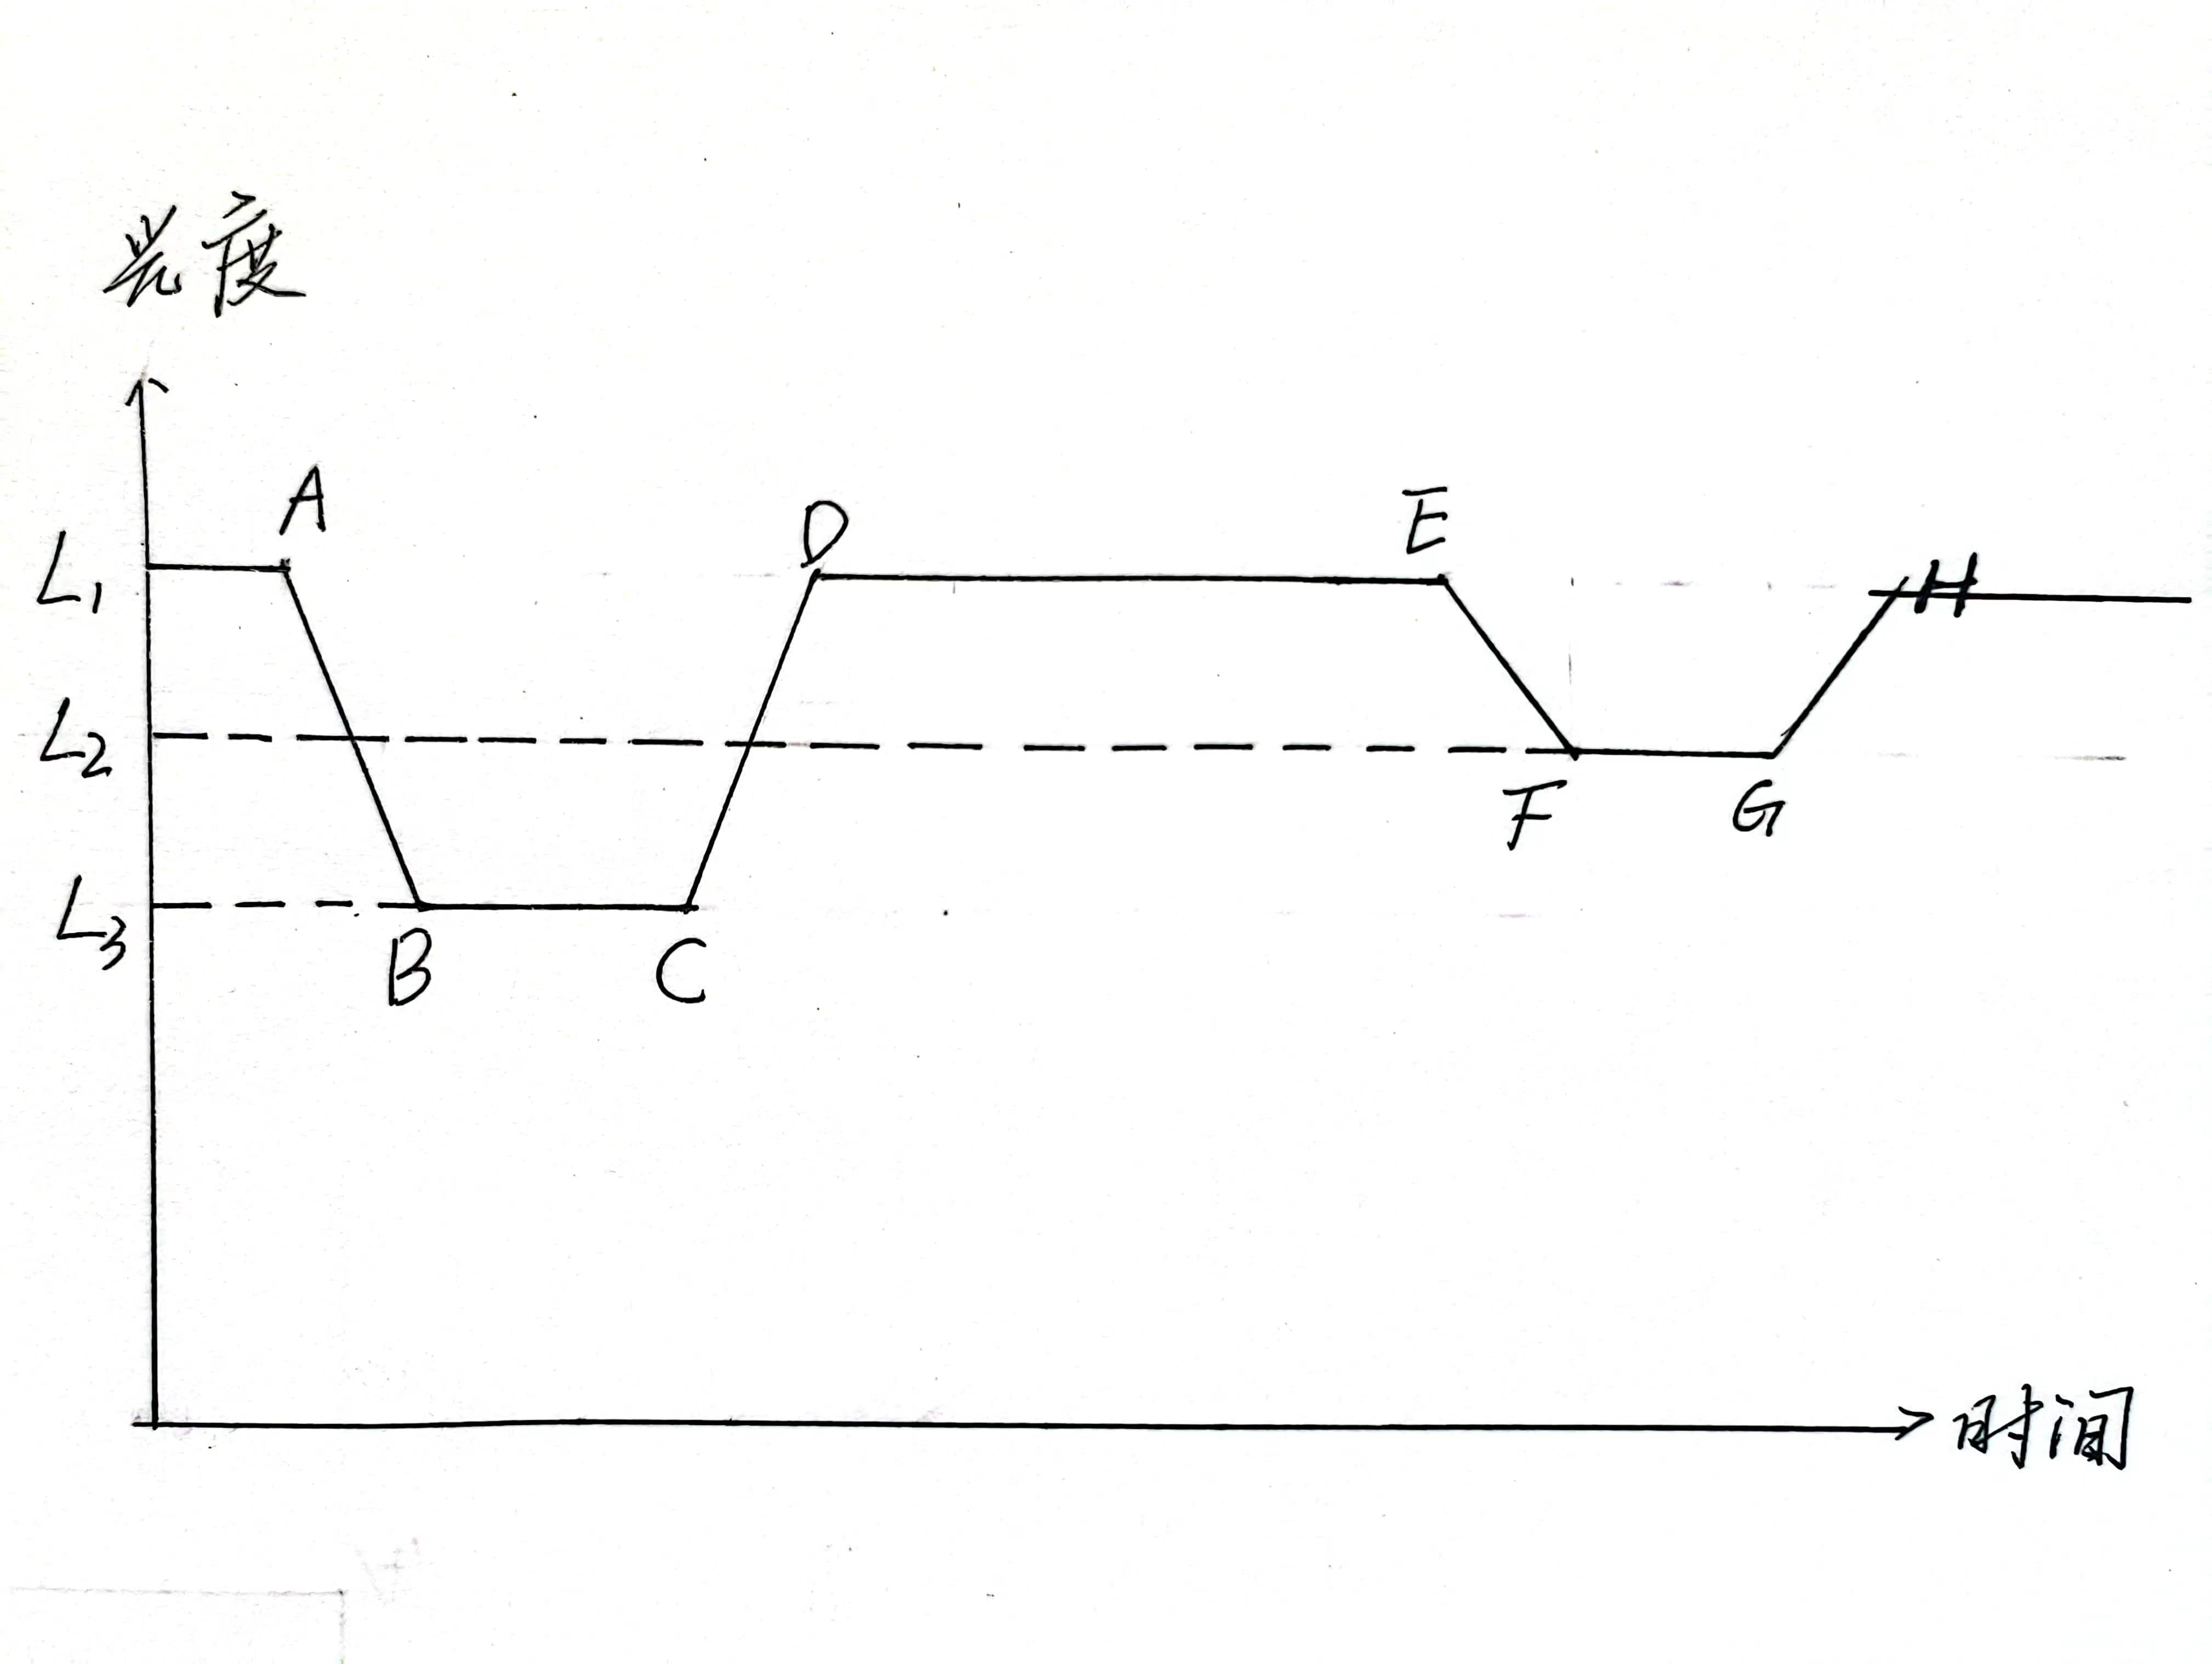
\includegraphics[width=10cm]{3_15.jpg}
	\caption{图三}
	%\label{fig:circuit-diagram}
\end{figure}
\noindent 解答:

\noindent $\left(1\right)$主星的轨道半径:
\begin{equation}
	a_{a}=\frac{Pv_{a}}{2\pi}
\end{equation}
次星的轨道半径:
\begin{equation}
	a_{b}=\frac{Pv_{b}}{2\pi}
\end{equation}
显然,可以得到关于两子星之间距离的等式:
\begin{equation}
	a=a_{a}+a_{b}
\end{equation}
主星的半径:
\begin{equation}
	R_{a}=\frac{2\pi a}{4P}\times (T_{e}+T_{t})
\end{equation}
次星的半径:
\begin{equation}
	R_{b}=\frac{2\pi a}{4P}\times (T_{e}-T_{t})
\end{equation}
注意到,轨道倾角$i=90^\circ$,根据开普勒第三定律可得:
\begin{equation}
	\frac{a^3\sin^3 i}{P^2}=M_{a}+M_{b}
\end{equation}
结合质心定义,应有:
\begin{equation}
	\frac{M_{a}}{M_{b}}=\frac{a_{a}}{a_{b}}
\end{equation}
以上各表达式联立可以得出:($R_{0}$和$M_{0}$分别表达太阳的半径和质量。)

主星的半径:$R_{a}=0.84R_{0}$
次星的半径:$R_{b}=0.61R_{0}$

主星的质量:$M_{1}=0.61M_{0}$
次星的质量:$M_{2}=0.46M_{0}$

\noindent  $\left(2\right)$ 恒星的质光关系为:
(本题解答根据向守平《天体物理概论》第81页做出。)
\begin{equation}
	\frac{L}{L_{0}}=(\frac{M}{M_{0}})^{\alpha}
\end{equation}
其中,$M \leq 0.3M_{0}$时,$\alpha=1.8$;

$0.3M_{0}<M\leq 3M_{0}$时,$\alpha=4.0$;

$M>3M_{0}$时,$\alpha=2.8$。

由此可得,$L_{a}=0.84^4L_{0}$,$L_{b}=0.64^4L_{0}$

\noindent 当两颗星的总光度为$L_{1}$时,两颗星没有发生互相遮挡。
\begin{equation}
	L_{1}=L_{a}+L_{b}=0.636L_{0}
\end{equation}
当两颗星的总光度为$L_{2}$时,主星将次星部分遮挡.
\begin{equation}
	L_{2}=L_{a}=0.498L_{0}
\end{equation}
当两颗星的总光度为$L_{3}$时,次星将主星部分遮挡,类比地球上的日环食,有:
\begin{equation}
	L_{3}=L_{2}+\frac{R_{1}^2-R_{2}^2}{R_{1}^2}\times L_{1}=0.374L_{0}
\end{equation}
\chapter{第三组}
\section{第一题}
\noindent 问题:在2020年秋分日(2020年9月22日北京时间21时31分秋分),某颗轨道半长轴4天文单位的小行星和太阳相距$180^\circ$。

$\left(1\right)$计算该小行星下次冲日的日期及此时在地球上观测,它的赤道坐标。

$\left(2\right)$使用口径150$mm$,焦距750$mm$的望远镜连接照相机使用赤道仪跟踪观测1小时,在焦平面上会留下多长的痕迹?

$\left(3\right)$若该小行星冲日时视星等为20等,表面反照率为5$\%$,在不考虑大气消光和大气折射的情况下,请计算该小行星的半径。

\noindent 解答:

$\left(1\right)$在2020年的秋分日,该小行星冲日。

$\left(\Rmnum{1}\right)$根据开普勒第三定律,
\begin{equation}
	\frac{a^3}{T^2}=1
\end{equation}
解得$T=8$年。上式中,轨道半长轴使用天文单位作为单位,所有轨道周期均以"年"作为单位。
根据会合周期的计算公式,:
\begin{equation}
	\frac{1}{t}=\frac{1}{T_{earth}}-\frac{1}{T}
\end{equation}
解得小行星和地球的会合周期$t=\frac{8}{7}$年。

显然,在2021年9月22日21时31分之后$\frac{1}{7}$年,该小行星再次冲日。

可以算出,该小行星再次冲日的日期时间为:2021年11月14日1时48分。

$\left(\Rmnum{2}\right)$
先计算在地球上观测,小行星的角速度。
S为太阳,$E_{1}$,$E_{2}$,$A_{1}$,$A_{2}$分别为地球、小行星在小行星冲日时及之后很短一段时间之后的位置。很明显,地球运行得更快。同时:

$E_{1}E_{2} \approx A_{1}E_{2}=v_{1}$,
$A_{1}A_{2}=v_{2}$,
$SE_{1}=a_{1}$,
$SA_{1}=a_{2}$
\begin{figure}[!h]
	\centering
	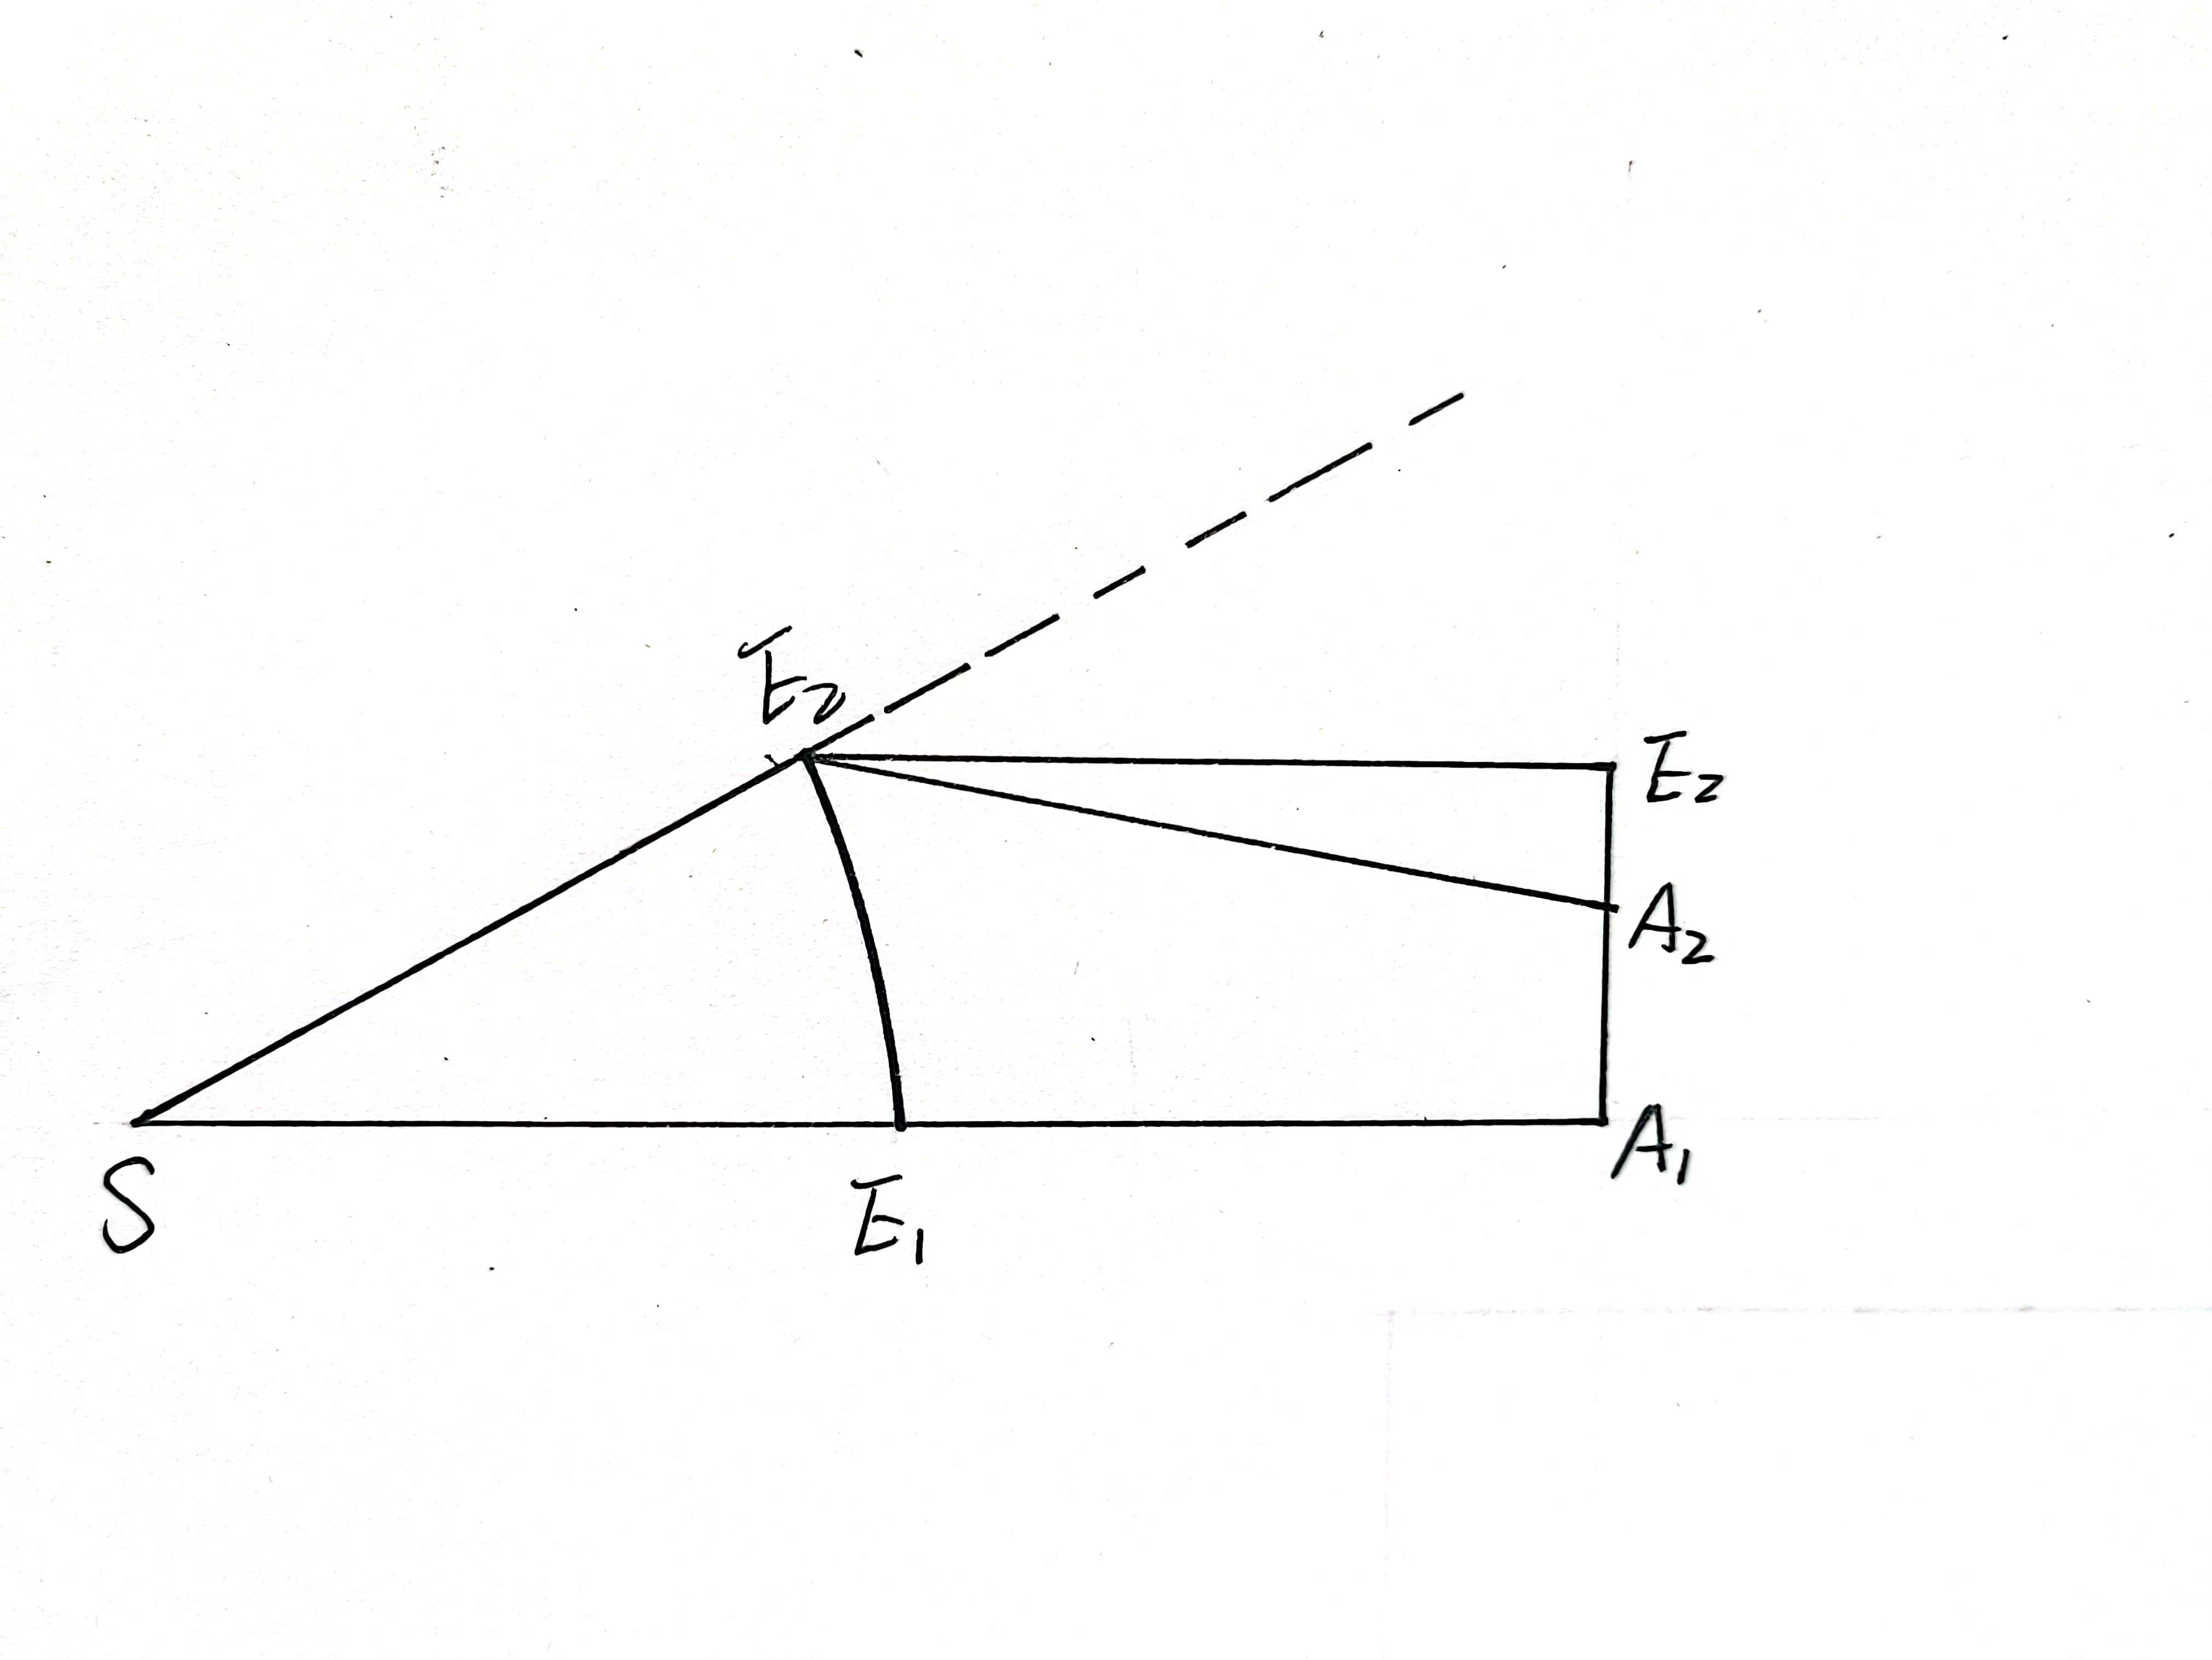
\includegraphics[width=12cm]{4_1.jpg}
	\caption{图四}
	%\label{fig:circuit-diagram}
\end{figure}
在地球上观测,小行星相对于背景恒星运动的角速度:
\begin{equation}
	\omega=\frac{v_{1}-v_{2}}{a_{2}-a_{1}}
\end{equation}
地球公转处的线速度:
\begin{equation}
	v_{1}=\frac{2\pi R_{earth}}{T_{earth}}
\end{equation}
小行星公转的线速度:
\begin{equation}
	v_{2}=\frac{2\pi R_{astroid}}{T_{astroid}}
\end{equation}
可以计算出,$\omega =-\frac{5\pi}{3}year^{-1}=-0.0342^{\prime\prime}/s$。
由题可知,该小行星始终在黄道面上,黄纬始终为零。小行星的黄经为$180^\circ-(\frac{360}{7})^\circ$。根据黄道坐标系和赤道坐标系的转换公式,有:

\begin{equation}
	\sin \lambda =\frac{\sin \delta}{\sin \varepsilon}
\end{equation}
\begin{equation}
	\cos \lambda =\cos \delta \cos \alpha
\end{equation}
经计算,小行星的赤道坐标:
$\alpha =3^{h}16^{m}0.70^{s}$
$\delta = 18^\circ 7^\prime 8.73^{\prime\prime}$

$\left(2\right)$
\begin{equation}
	x=f\tan \theta =750mm\times \sin(0.0342\times 3600)=4.48mm
\end{equation}

$\left(3\right)$
记$W_{M}$,$W_{A}$分别为月球和小行星处的太阳常数,$\alpha_{M}$和$\alpha_{A}$分别为月球和小行星的表面反照率(取平均值),$S_{M}$和$S_{A}$分别为月球和小行星的表面积,$I_{M}$和$I_{A}$分别为地球上接收到的辐射流量。
\begin{equation}
	I_{M}=\frac{W_{M}\alpha_{M}S_{M}}{2\pi D_{M}^2}
\end{equation}
\begin{equation}
	I_{A}=\frac{W_{A}\alpha_{A}S_{A}}{4\pi D_{A}^2}
\end{equation}
\begin{equation}
	\frac{W_{M}}{W_{A}}=(\frac{D_{M}}{D_{A}})^2
\end{equation}

\begin{equation}
	\Delta m=m_{M}-m_{A}=-2.5\lg \frac{I_{M}}{I_{A}}
\end{equation}
以上各表达式联立,可得小行星的半径$R_{astroid}=752km$。
\section{第二题}
\noindent 问题:冬季星空中的重要梅西耶天体——疏散星团M45距离我们128秒差距。以下计算请忽略大气消光。

$\left(1\right)$昴星团的角直径为$2^\circ$,请估算线直径。

某颗$\Rmnum{1}a$型超新星和我们的距离是昴星团和我们之间距离的10倍。经检测,该超新星光度极大值是爆发之前的$10^{12}$倍。

$\left(2\right)$对此超新星的光谱分析表明,在光极大时,理论波长为6335埃的一次电离硅波长变位7335埃。请据此估算哈勃常数。

$\left(3\right)$在考虑星际消光的条件下,假设星光每传播1秒差距会使视星等下降0.02等。请求出此超新星在光极大时在地球上观测的视星等。

$\left(4\right)$爆发之前,该超新星的光度是太阳的一万倍,半径是太阳的四倍。估算得出此恒星寿命约为太阳寿命的十分之一。

$\left(4-a\right)$求其爆发之前的表面有效温度。

$\left(4-b\right)$求其辐射最为猛烈时的波长值并给出此时单个光子携带的能量。

$\left(4-c\right)$请根据本题信息推测(提示:利用赫罗图。)它在爆发前可能的光谱型(哈佛分类法只需要给出主型)并论证。

$\left(5\right)$请尽可能详尽地写出超新星的分类及对应标准。


\noindent 解答:

$\left(1\right)$根据几何关系,M45的视直径:
\begin{equation}
	d=2L\tan \theta =4.36pc
\end{equation}
$\left(2\right)$
\begin{equation}
	z=\frac{v}{c}=\frac{H_{0}D}{c}=\frac{\lambda_{2}-\lambda_{1}}{\lambda_{1}}
\end{equation}
得出:$H_{0}=3.685\times 10^{-5}km/s/Mpc$
但是该超新星的距离过近,哈勃定律不成立。

$\left(3\right)$
根据常识,所有的$\Rmnum{1}a$型超新星在光度极大时的绝对星等均为$-19.3^m$。不考虑星际消光,有:
\begin{equation}
	m-M=5\lg r-5
\end{equation}

\begin{equation}
	m_{0}^{\prime}=m+\Delta m=m+kr
\end{equation}
以上两式联立解得$m_{0}=16.836^m$
$\left(4\right)$

$\left(4-a\right)$
根据斯特藩-玻尔兹曼定律(本小问中带有角标的表达太阳对应量。)
\begin{equation}
	\frac{L}{L_{0}}=(\frac{R}{R_{0}})^2\times(\frac{L}{L_{0}})^4
\end{equation}
解得$T=5T_{0}=29000K$

$\left(4-b\right)$

辐射最猛烈的波长:
\begin{equation}
	\lambda_{max}=\frac{b}{T}=\frac{0.29}{29000}cm=10^{-7}m
\end{equation}
单个光子携带的能量:
\begin{equation}
	E=\frac{hc}{\lambda_{max}}=1.986\times 10^{-18}J
\end{equation}

$\left(4-c\right)$该恒星为O型星。本判断根据《天文学新概论》第四版155页表格做出。

$\left(5\right)$本题具体作答略。见刘学富《基础天文学》280-281页和
肖兴华、李宗伟《天体物理学》(第二版)207-215页。

\section{第三题(本题因历史原因不给出解答。)}
有一颗距离我们200秒差距,质量为100倍太阳质量的主序星,其表面温度为29000开尔文,我们刚好可以使用一望远镜看到。后来这颗恒星演化到了红巨星分支,表面有效温度下降到原来的三分之一,半径膨胀到原来的一百倍。同样假设假设星光每传播1秒差距会使视星等下降0.02等。已知该主序星的半径是太阳半径的十倍。

$\left(1\right)$此时,若我们的后代用同样的望远镜也观测到了这颗红巨星,求这颗主序星距离可能的最大值。

$\left(2\right)$
该恒星是一颗脉动变星,其半径的变化量为百分之五。求在地球上观测,该恒星星等的取值范围。
\section{第四题(本题因历史原因不给出解答。)}
现考虑一个质量为太阳质量的1000倍,半径10秒差距,温度10开尔文的星云。

$\left(1\right)$该星云能够收缩吗?请通过计算给出论证。

$\left(2\right)$在此时,该星云的自转周期为一百万年。它的尺度收缩至太阳系尺度(50天文单位)时,求自转周期。已知若一气体云能够收缩,内部气体的平均速度必须小于星云逃逸速度的一半。
\section{第五题(本题因历史原因不给出解答。)}
火星曾多次出现在CNAO的题目中。2018年7月,有一只企鹅在圣彼得堡的冬宫广场看到了冲日的火星。考虑大气消光、大气折射,忽略火星的轨道倾角。同时假设月球和火星只将太阳光反射到面向太阳的半个天球,且其亮度处处相等。

$\left(1\right)$
求在圣彼得堡观测,火星大冲时地平高度的最值。

$\left(2\right)$
在考虑火星轨道偏心率时,求火星大冲时的视星等。




\chapter{本文档中各题目来源}
\section{第一组题目}
第一题:改编自2004年CNAO决赛第十三题。

第二题:改编自2003年CNAO决赛第五题。

第三题:改编自第七届IAO压轴题。

第四题:原创。

第五题:来自《天文奥赛指南》。

第六题:原创。

第七题:原创。

第八题:原创。灵感来自2004年CNAO决赛第11题。

第九题:2008年IAO高年组第二题。

第十题:1999年IAO第三题。
\section{第二组题目}
第一题:吉林大学天文协会。已获授权。

第二题:2005年IAO高年组第五题

第三题:2003年CNAO决赛第四题

第四题:改编自2003年CNAO决赛第七题

第五题:吉林大学天文协会。已获授权。

第六题:2006年CNAO决赛第十三题。题目中图像被略去。

第七题:改编自2006年俄罗斯天文通讯赛第六题。

第八题:2008年俄罗斯天文通讯赛第八题。

第九题:改编自《天文奥赛指南》158页第九题。

第十题:改编自《天文奥赛指南》158页第八题。

第十一题:改自《天文奥赛指南》157页第6题。

第十二题:2006年俄罗斯天文通讯赛第五题。

第十三题:2006年俄罗斯天文通讯赛第八题。

第十四题:2006年APAO高年组第六题。

第十五题:2008IOAA长问题第一题。

\section{第三组题目}
第三组题目中,除第一题改编自2006年CNAO高年组第十五题外,余下各题目均为原创。
\end{document}          
